\documentclass[12pt]{article}
\usepackage{savetrees}
\title{Google Modified Cardboard, 22- 25 December 2014}
\author{Dolly Shahani, Deval Shah, Aparajita Sahoo}
\usepackage{indentfirst}
\usepackage{graphicx}
\usepackage{setspace}

\begin{document}
\maketitle
Eye modular Prototype design using 1 camera.
Thing to Incorporate 

  1. lens 

  2. LED (White and IR)
	
  3. Camera (IR filter removed)

  4. Beamsplitter 

This is a two camera prototype. The dimensions of the google cardboard prototype are changed according to the type of lens which is going to fit in. The lens used is convexo-convex which has a focal length of 55mm. We change the dimensions according to the lens going to be fitted, and the beam splitter which is going to be aligned at an angle of 45 degrees, in front of lens. The IR and white LEDs are fitted on both the sides of cardboard so that a proper illumination is obtained to capture the lens onto the camera. \\
Steps:

1. We first tried to make a google cardboard prototype, and fixed LEDs (white and IRs), beam splitter and camera to see their positions. 

2. We were able to capture the exact location of eye. The eye was observed because of light deflected due to beam splitter.

3. The location and dimensions for lens and box were fixed.

4. The initial Google cardboard design was modified. That was done with the help of solidworks. 

5. The pdf was printed and new modified 
cardboard was formed. \\

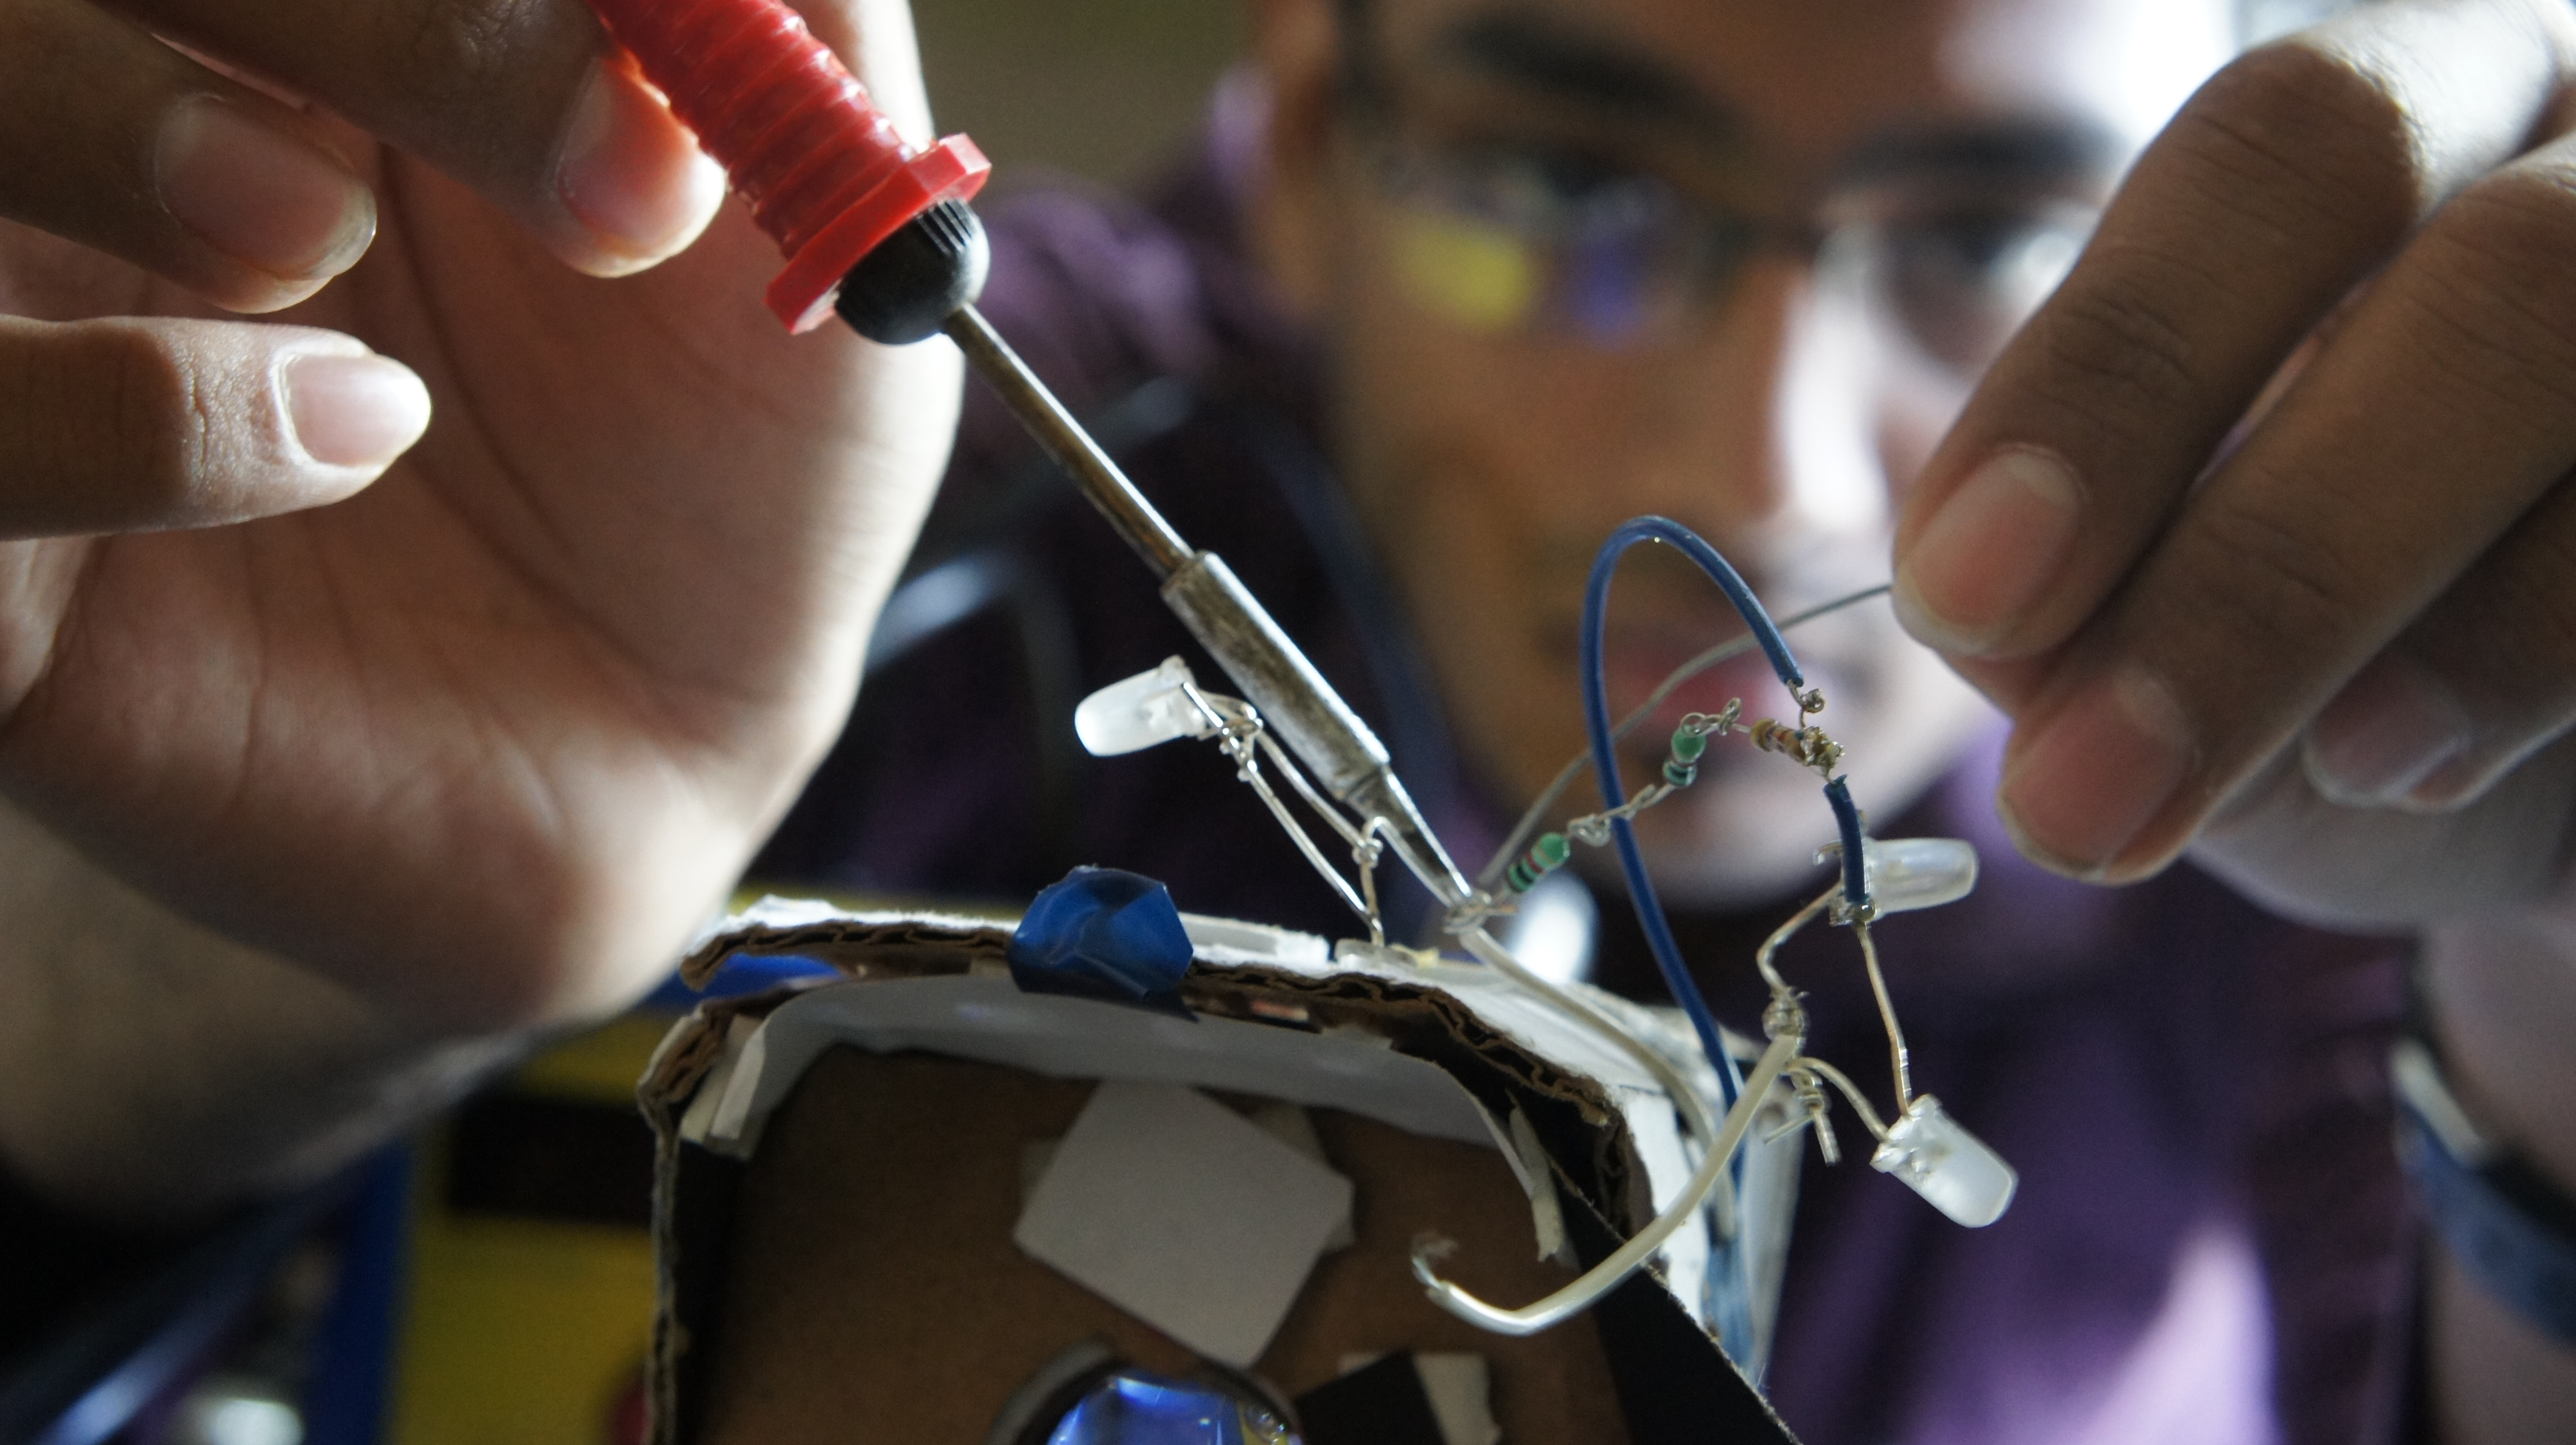
\includegraphics[width=8cm]{gh}
\includegraphics[width=8cm]{DSC03893}

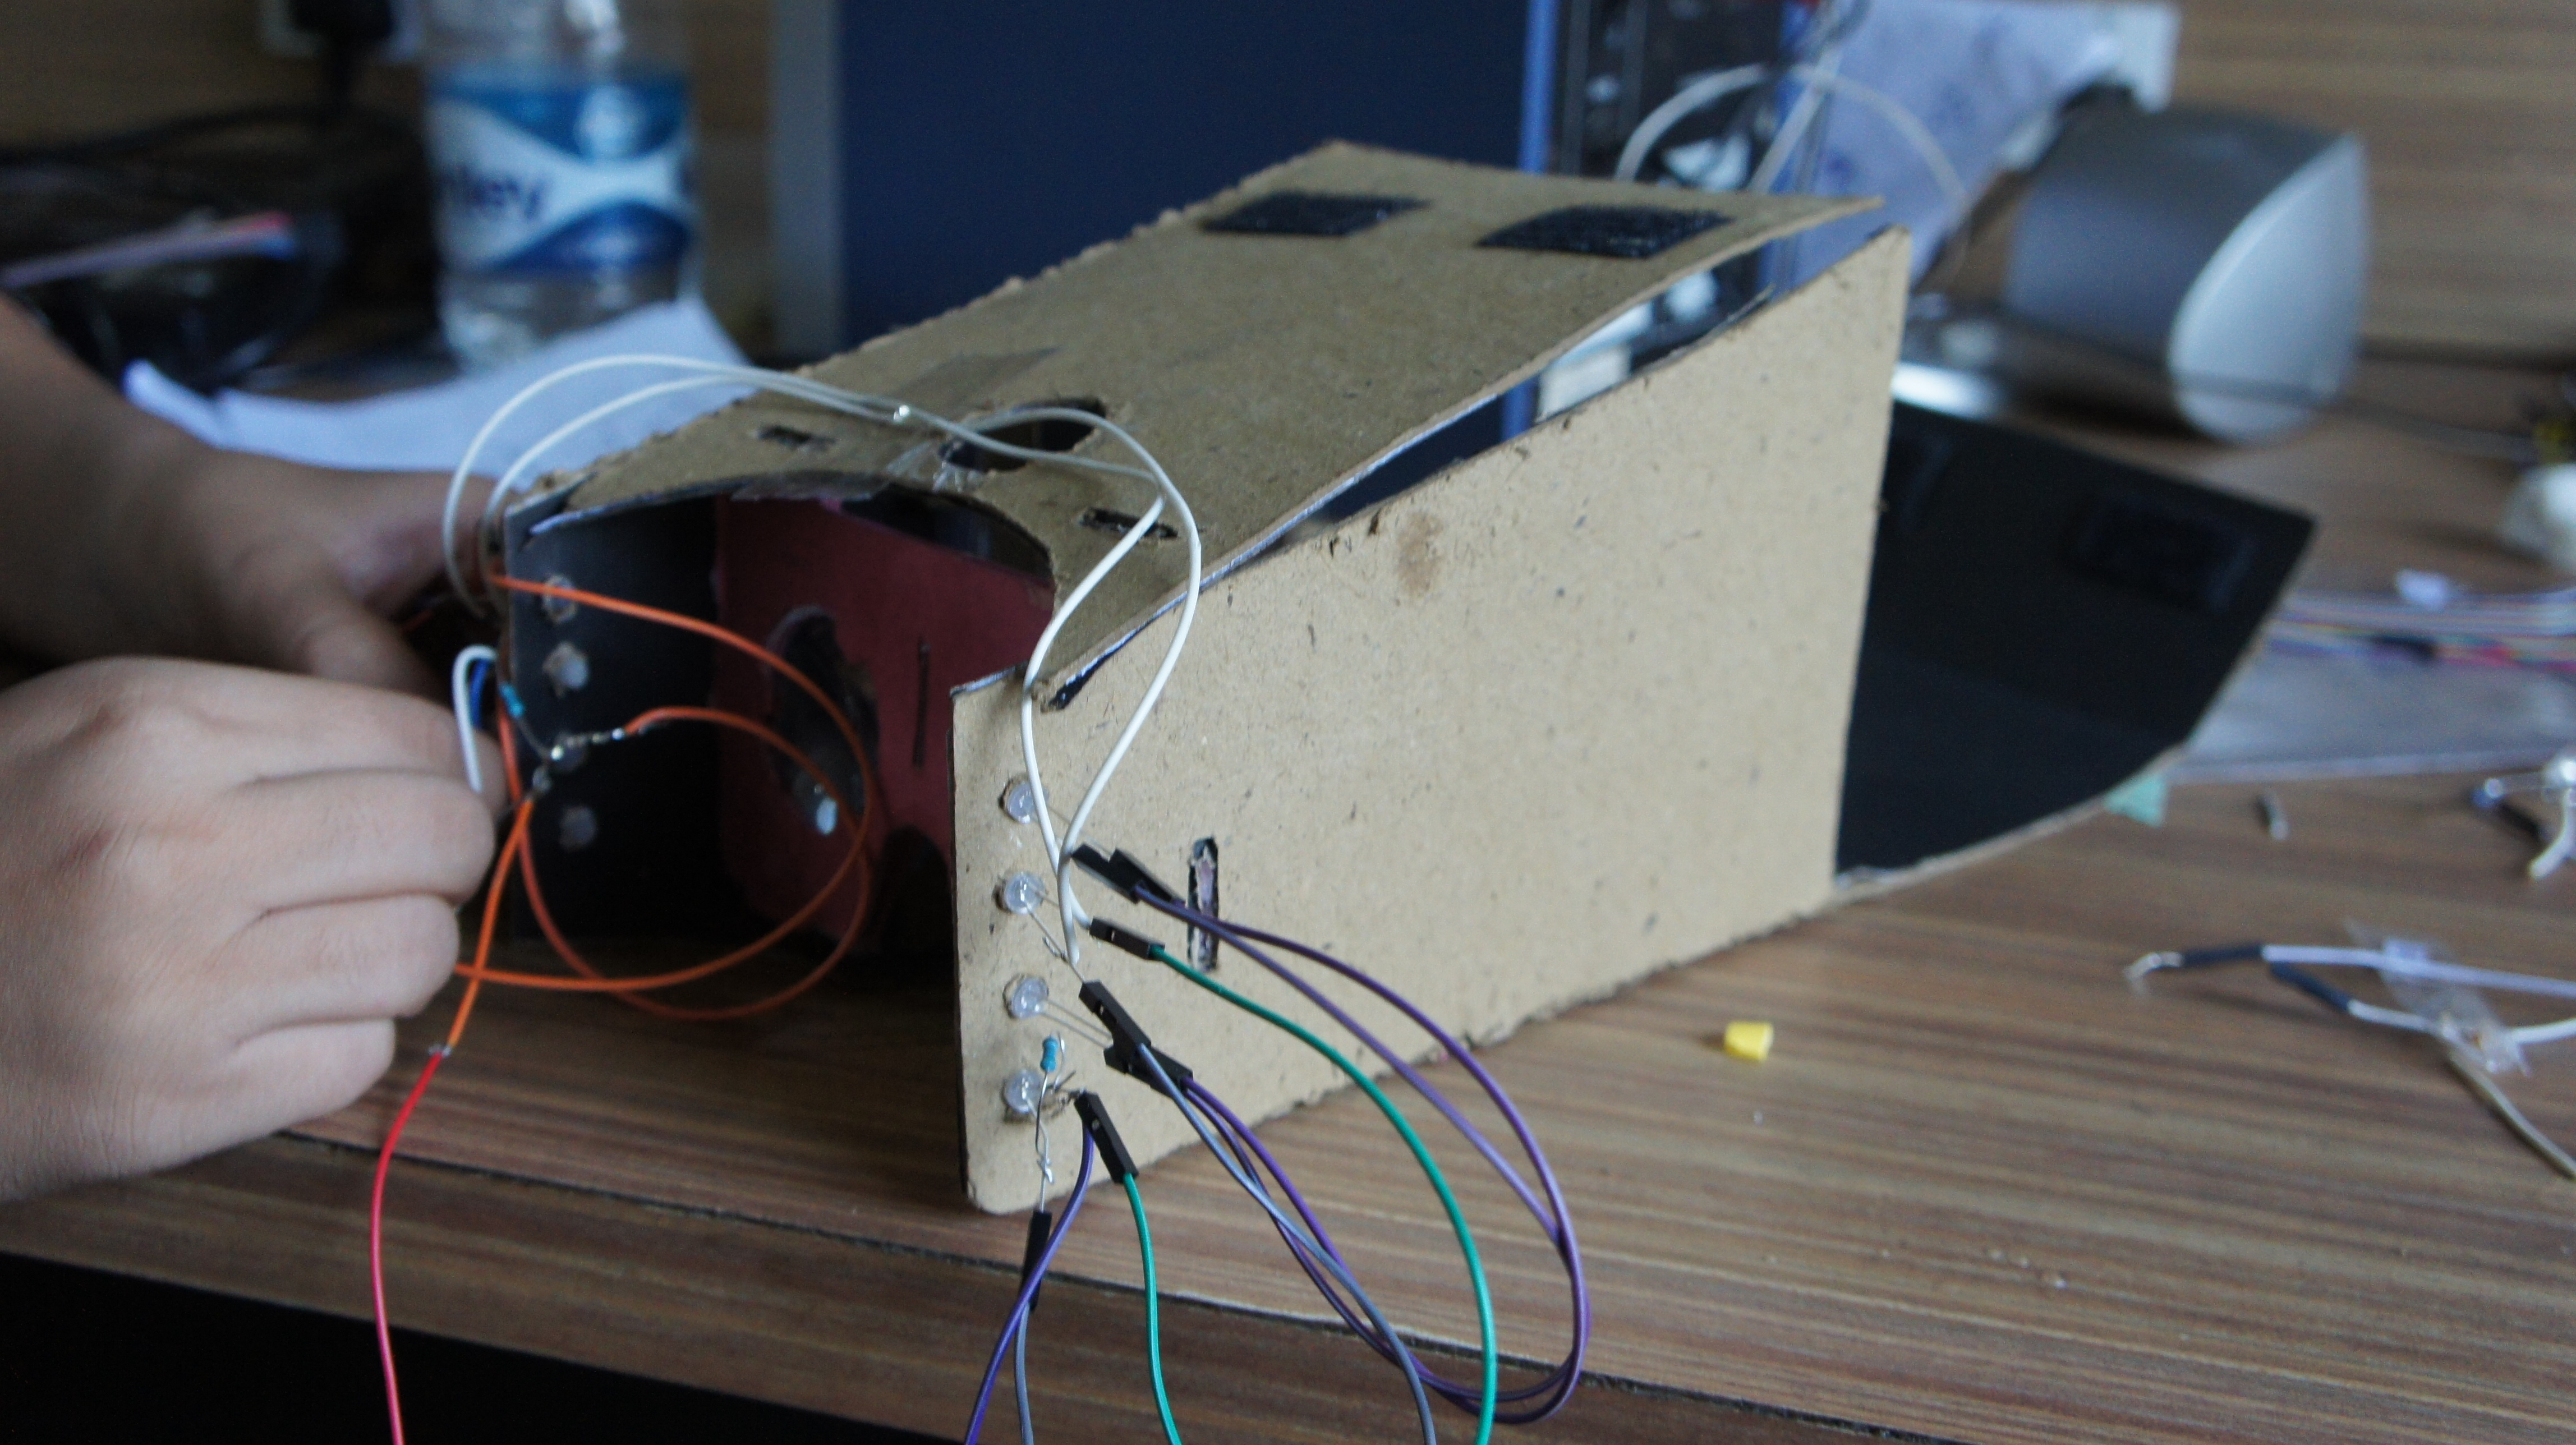
\includegraphics[width=8cm]{DSC03895} 
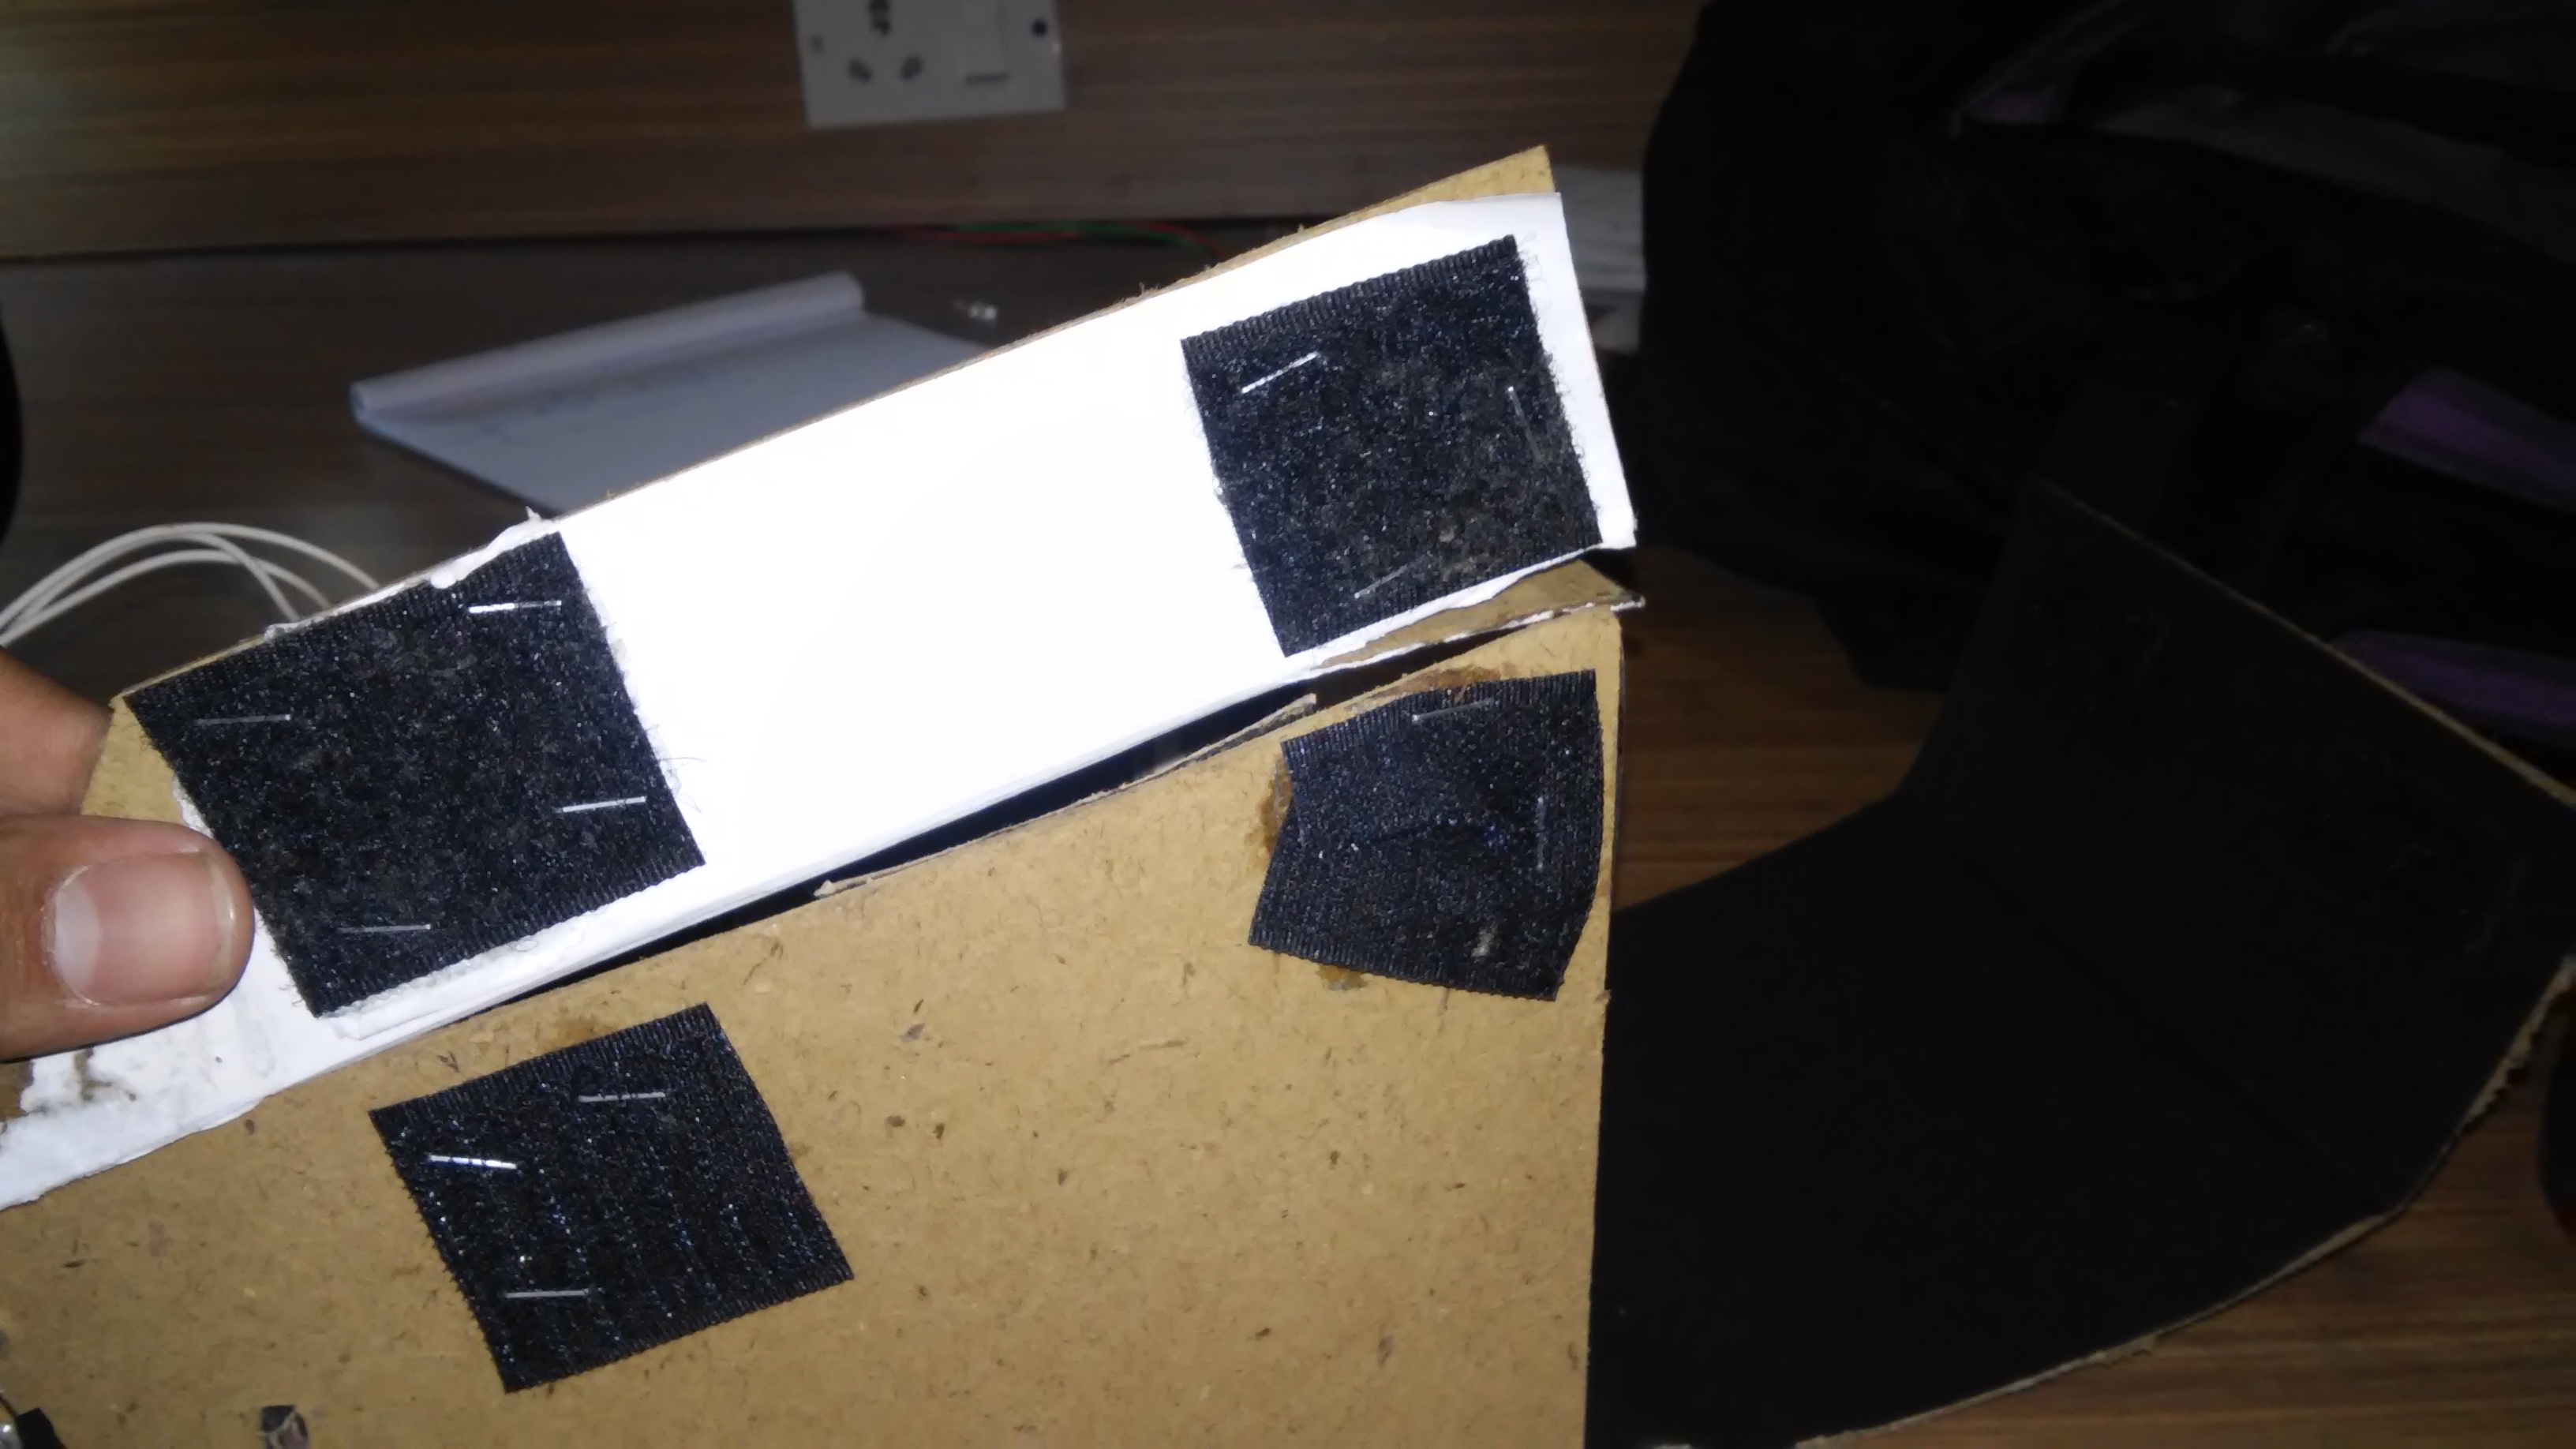
\includegraphics[width=8cm]{20141225_162318} 


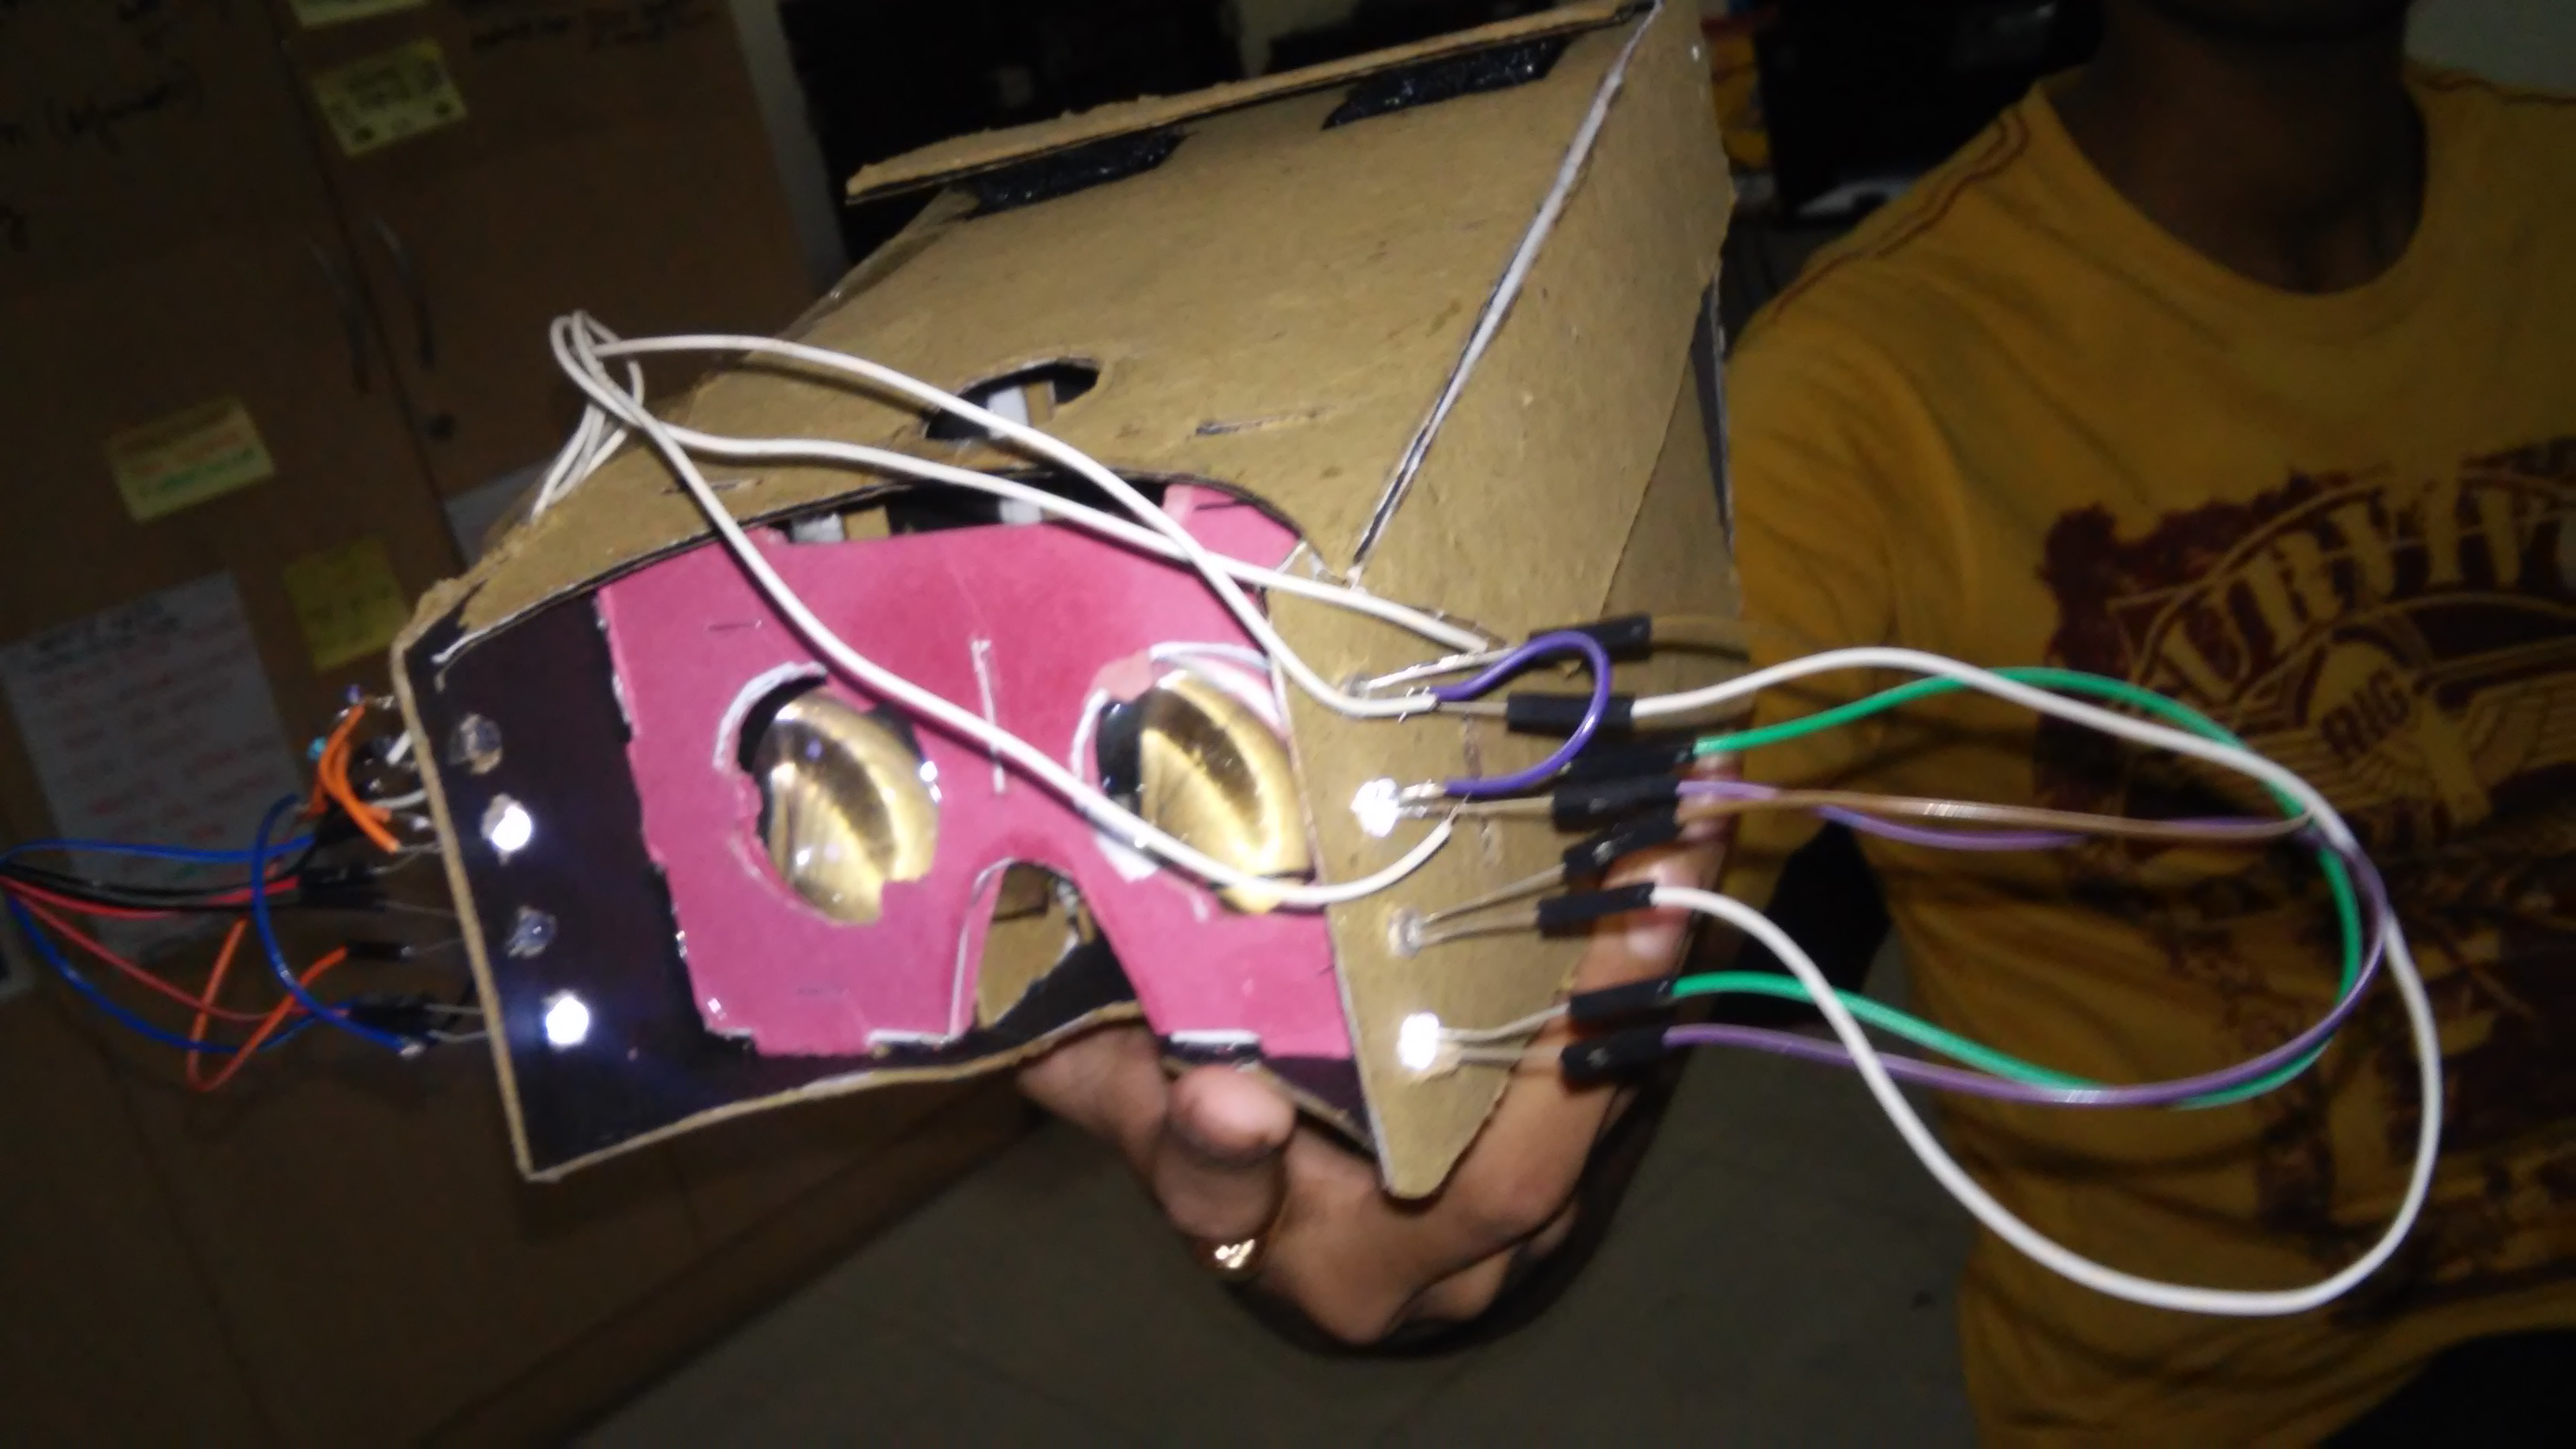
\includegraphics[width=8cm]{20141225_172947} 
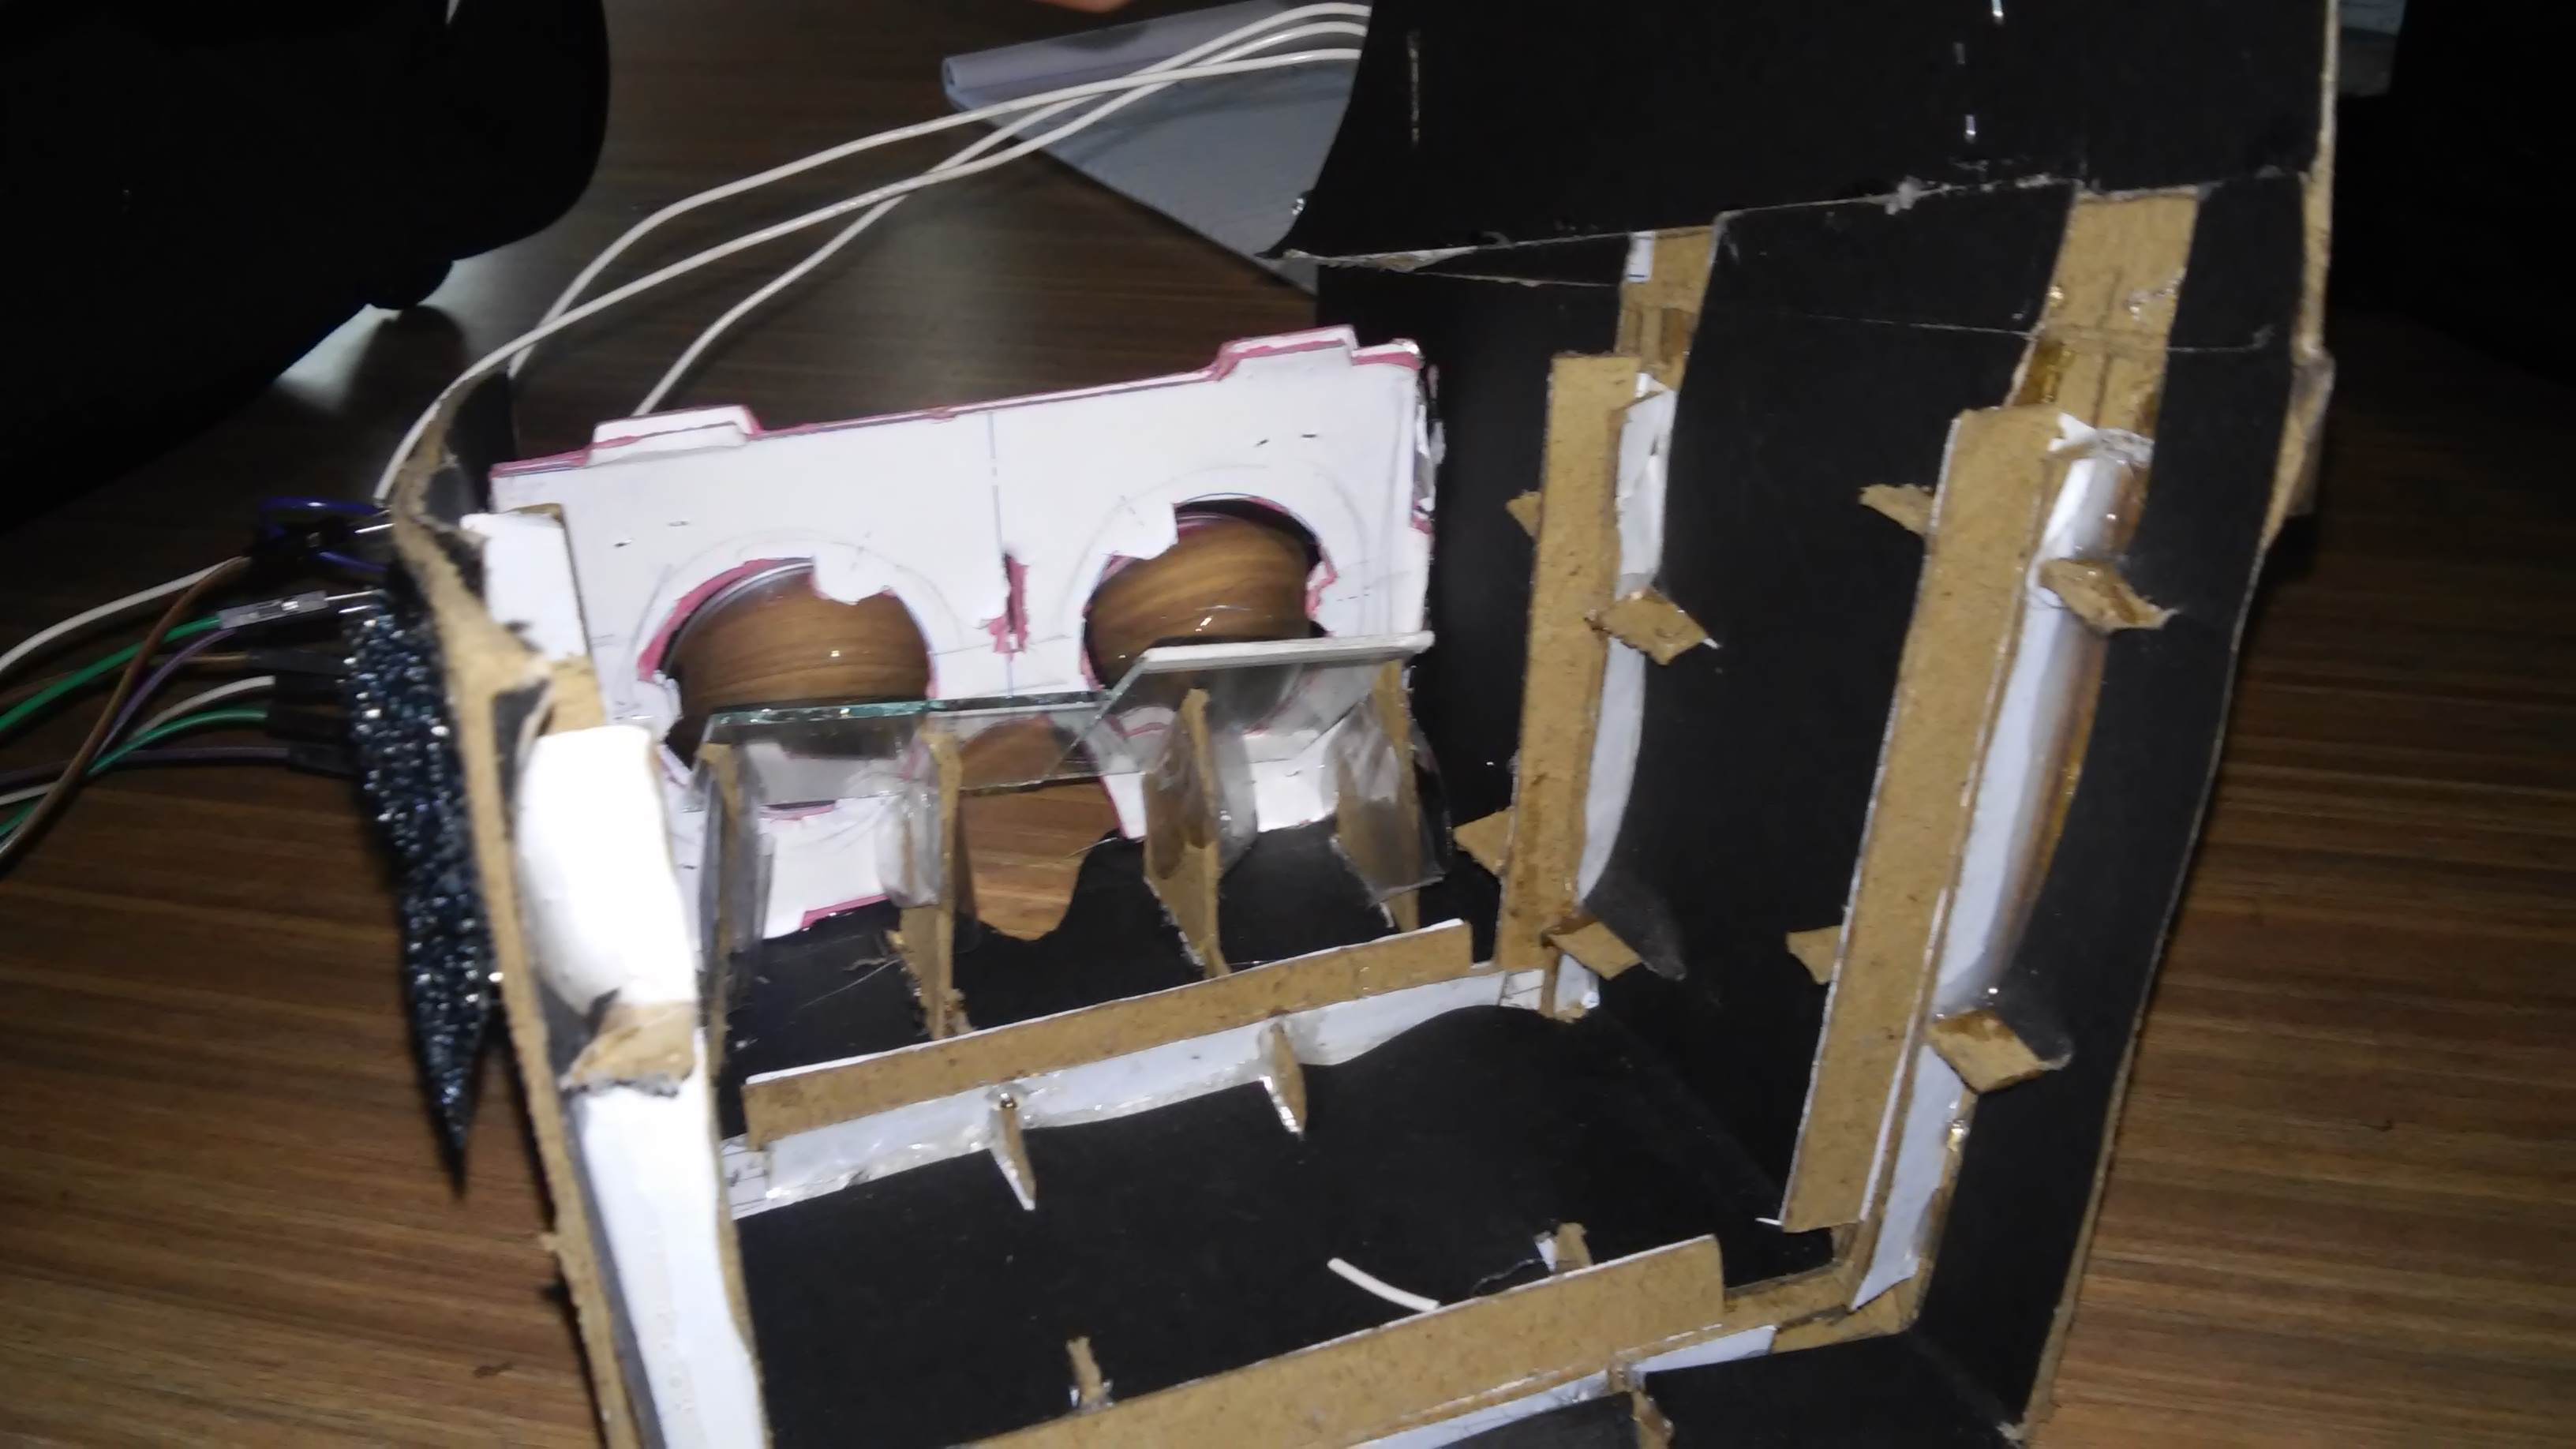
\includegraphics[width=8cm]{20141225_162310} \\


This prototype uses lens of focal length 5.5cm, and has two slots for fitting in LCDs. We have fitted 2 White LEDs and 2 IR LEDs altenatively on each side. The inside of box is covered with black chart paper so that no reflections are obtained.A camera is attached at the top  and 2 beam splitters are fixed at the base which are inclined at angle of 45 degree. It is a box which can be opened from upper surface (as shown in figure, using velcro) which allows us to inspect and experiment the inside of the box properly, the fitting of beam splitters, camera with proper alignment. \\
A  9V battery, 2 560 ohms, 2 330 ohm resistors, 8 LEDS are fixed as shown as figure.\\




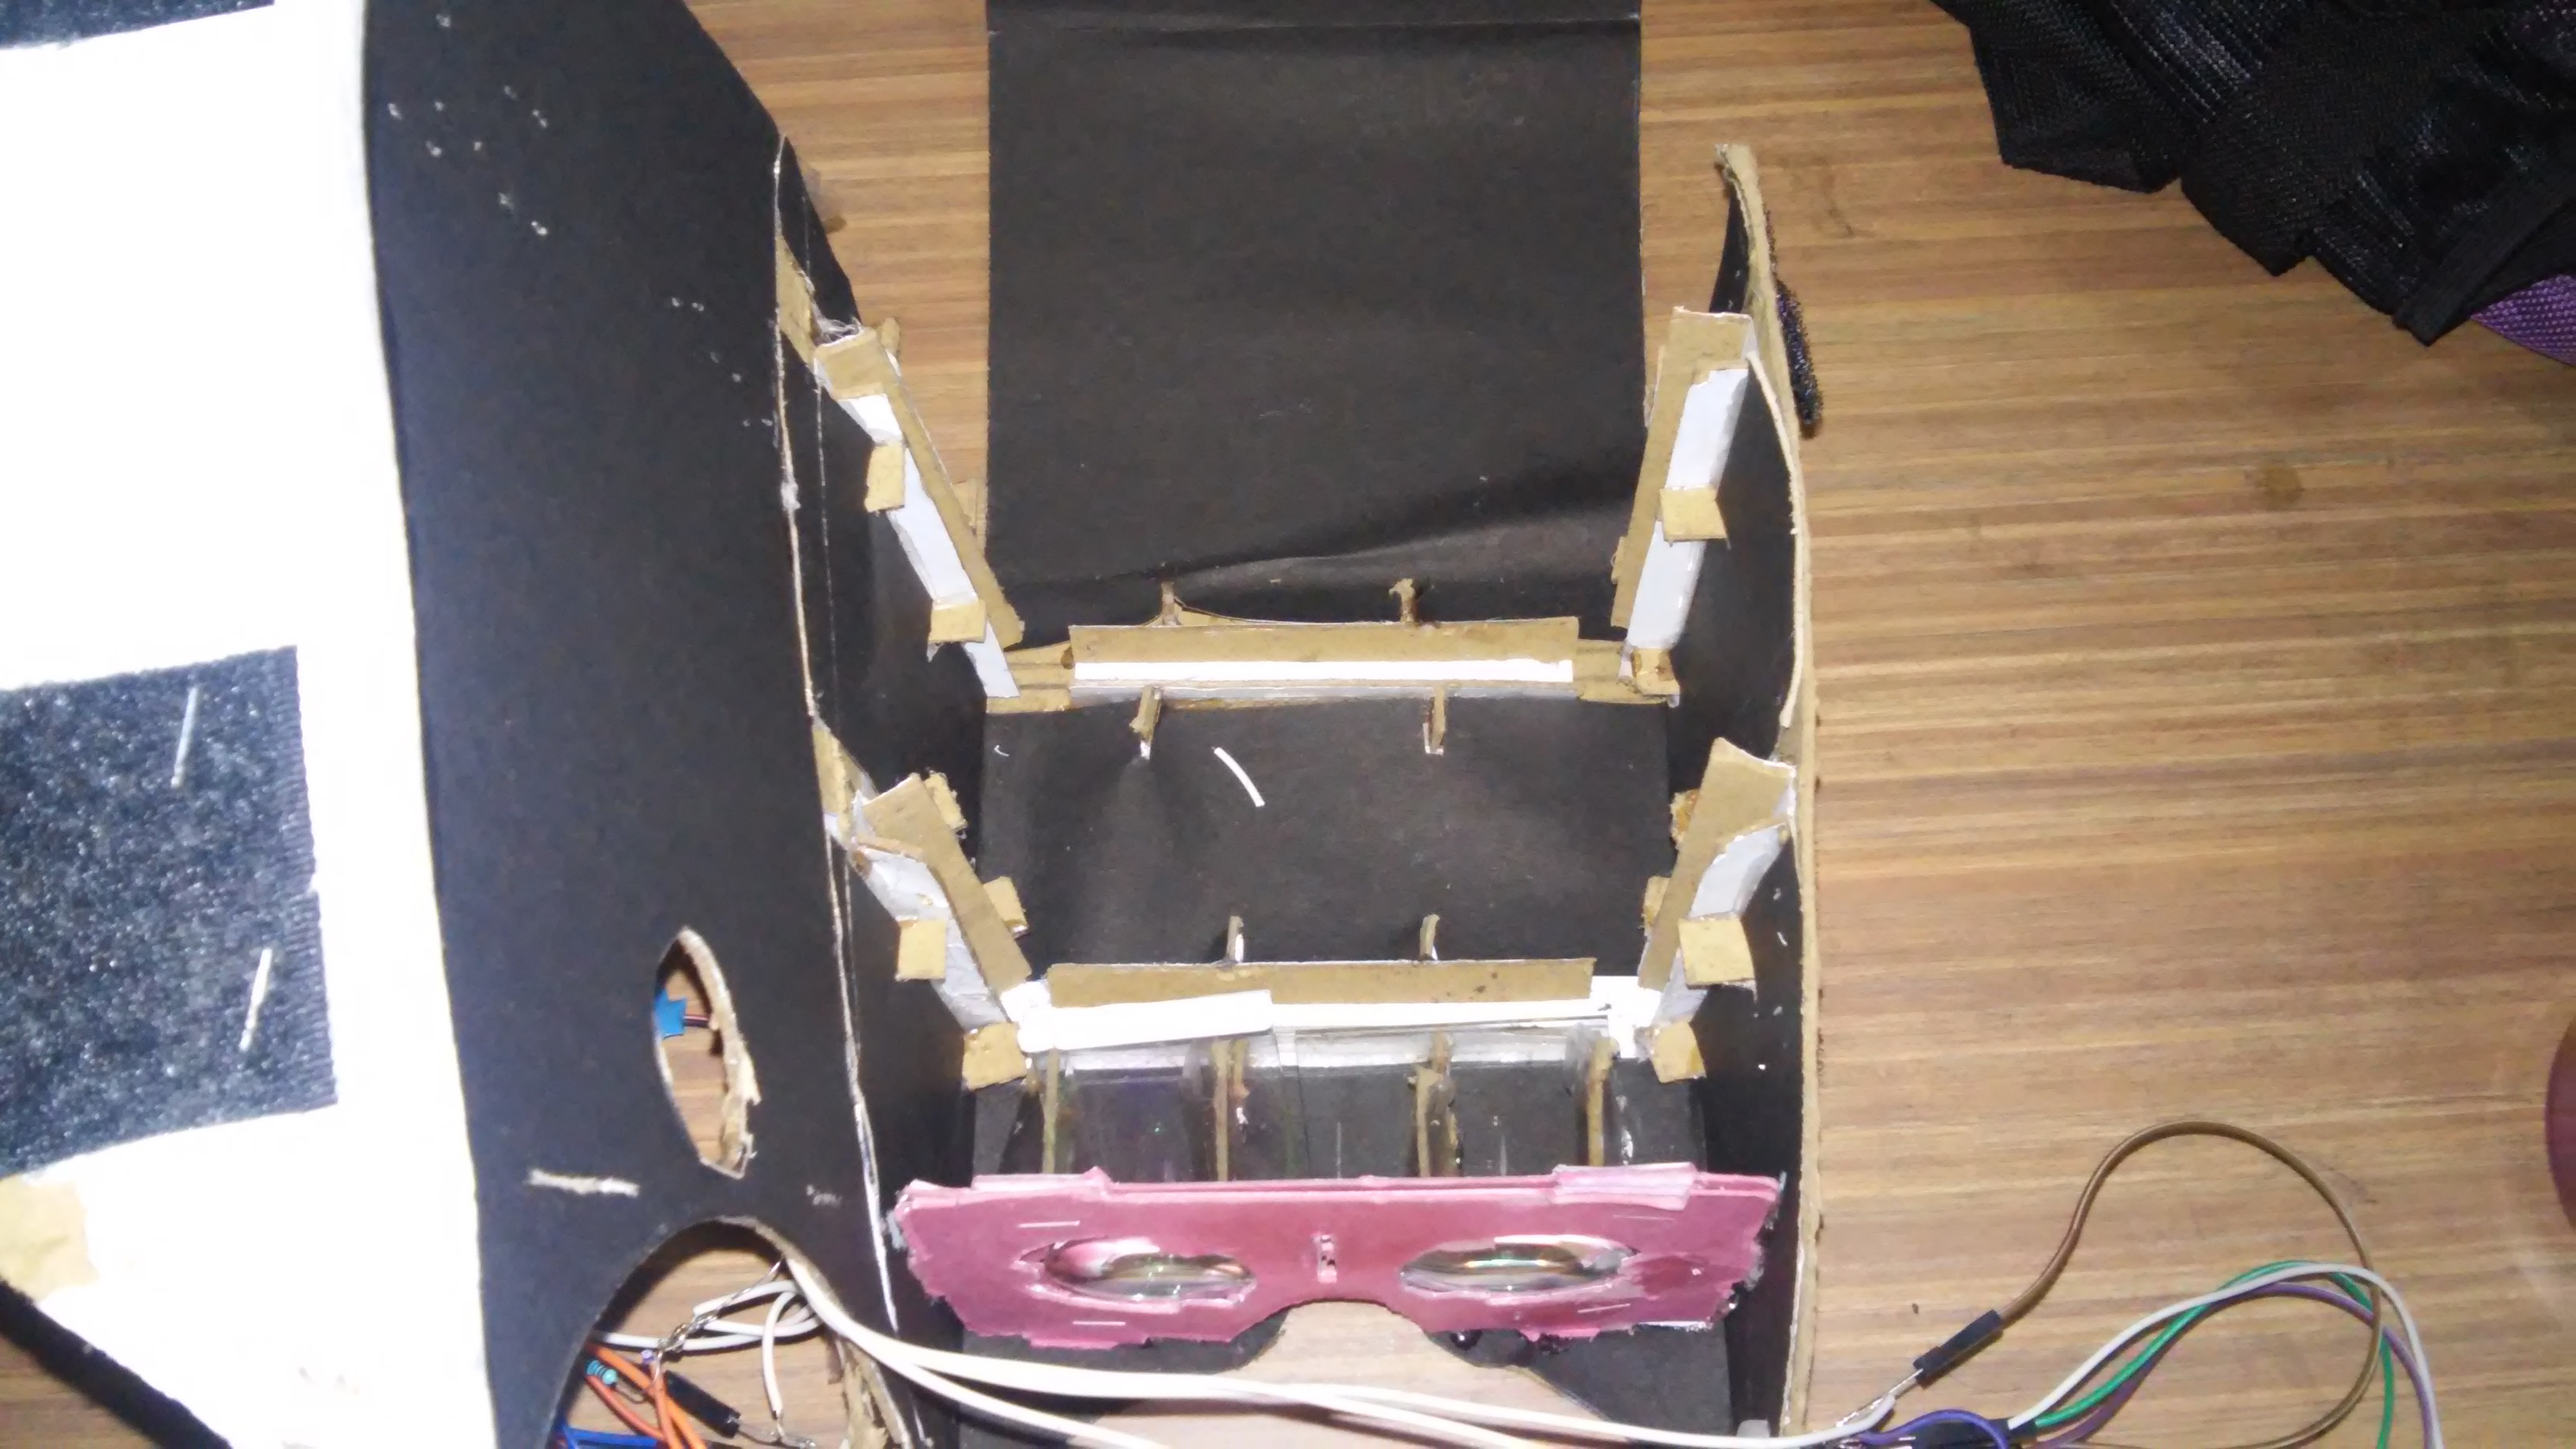
\includegraphics[width=8cm]{20141225_162257} 
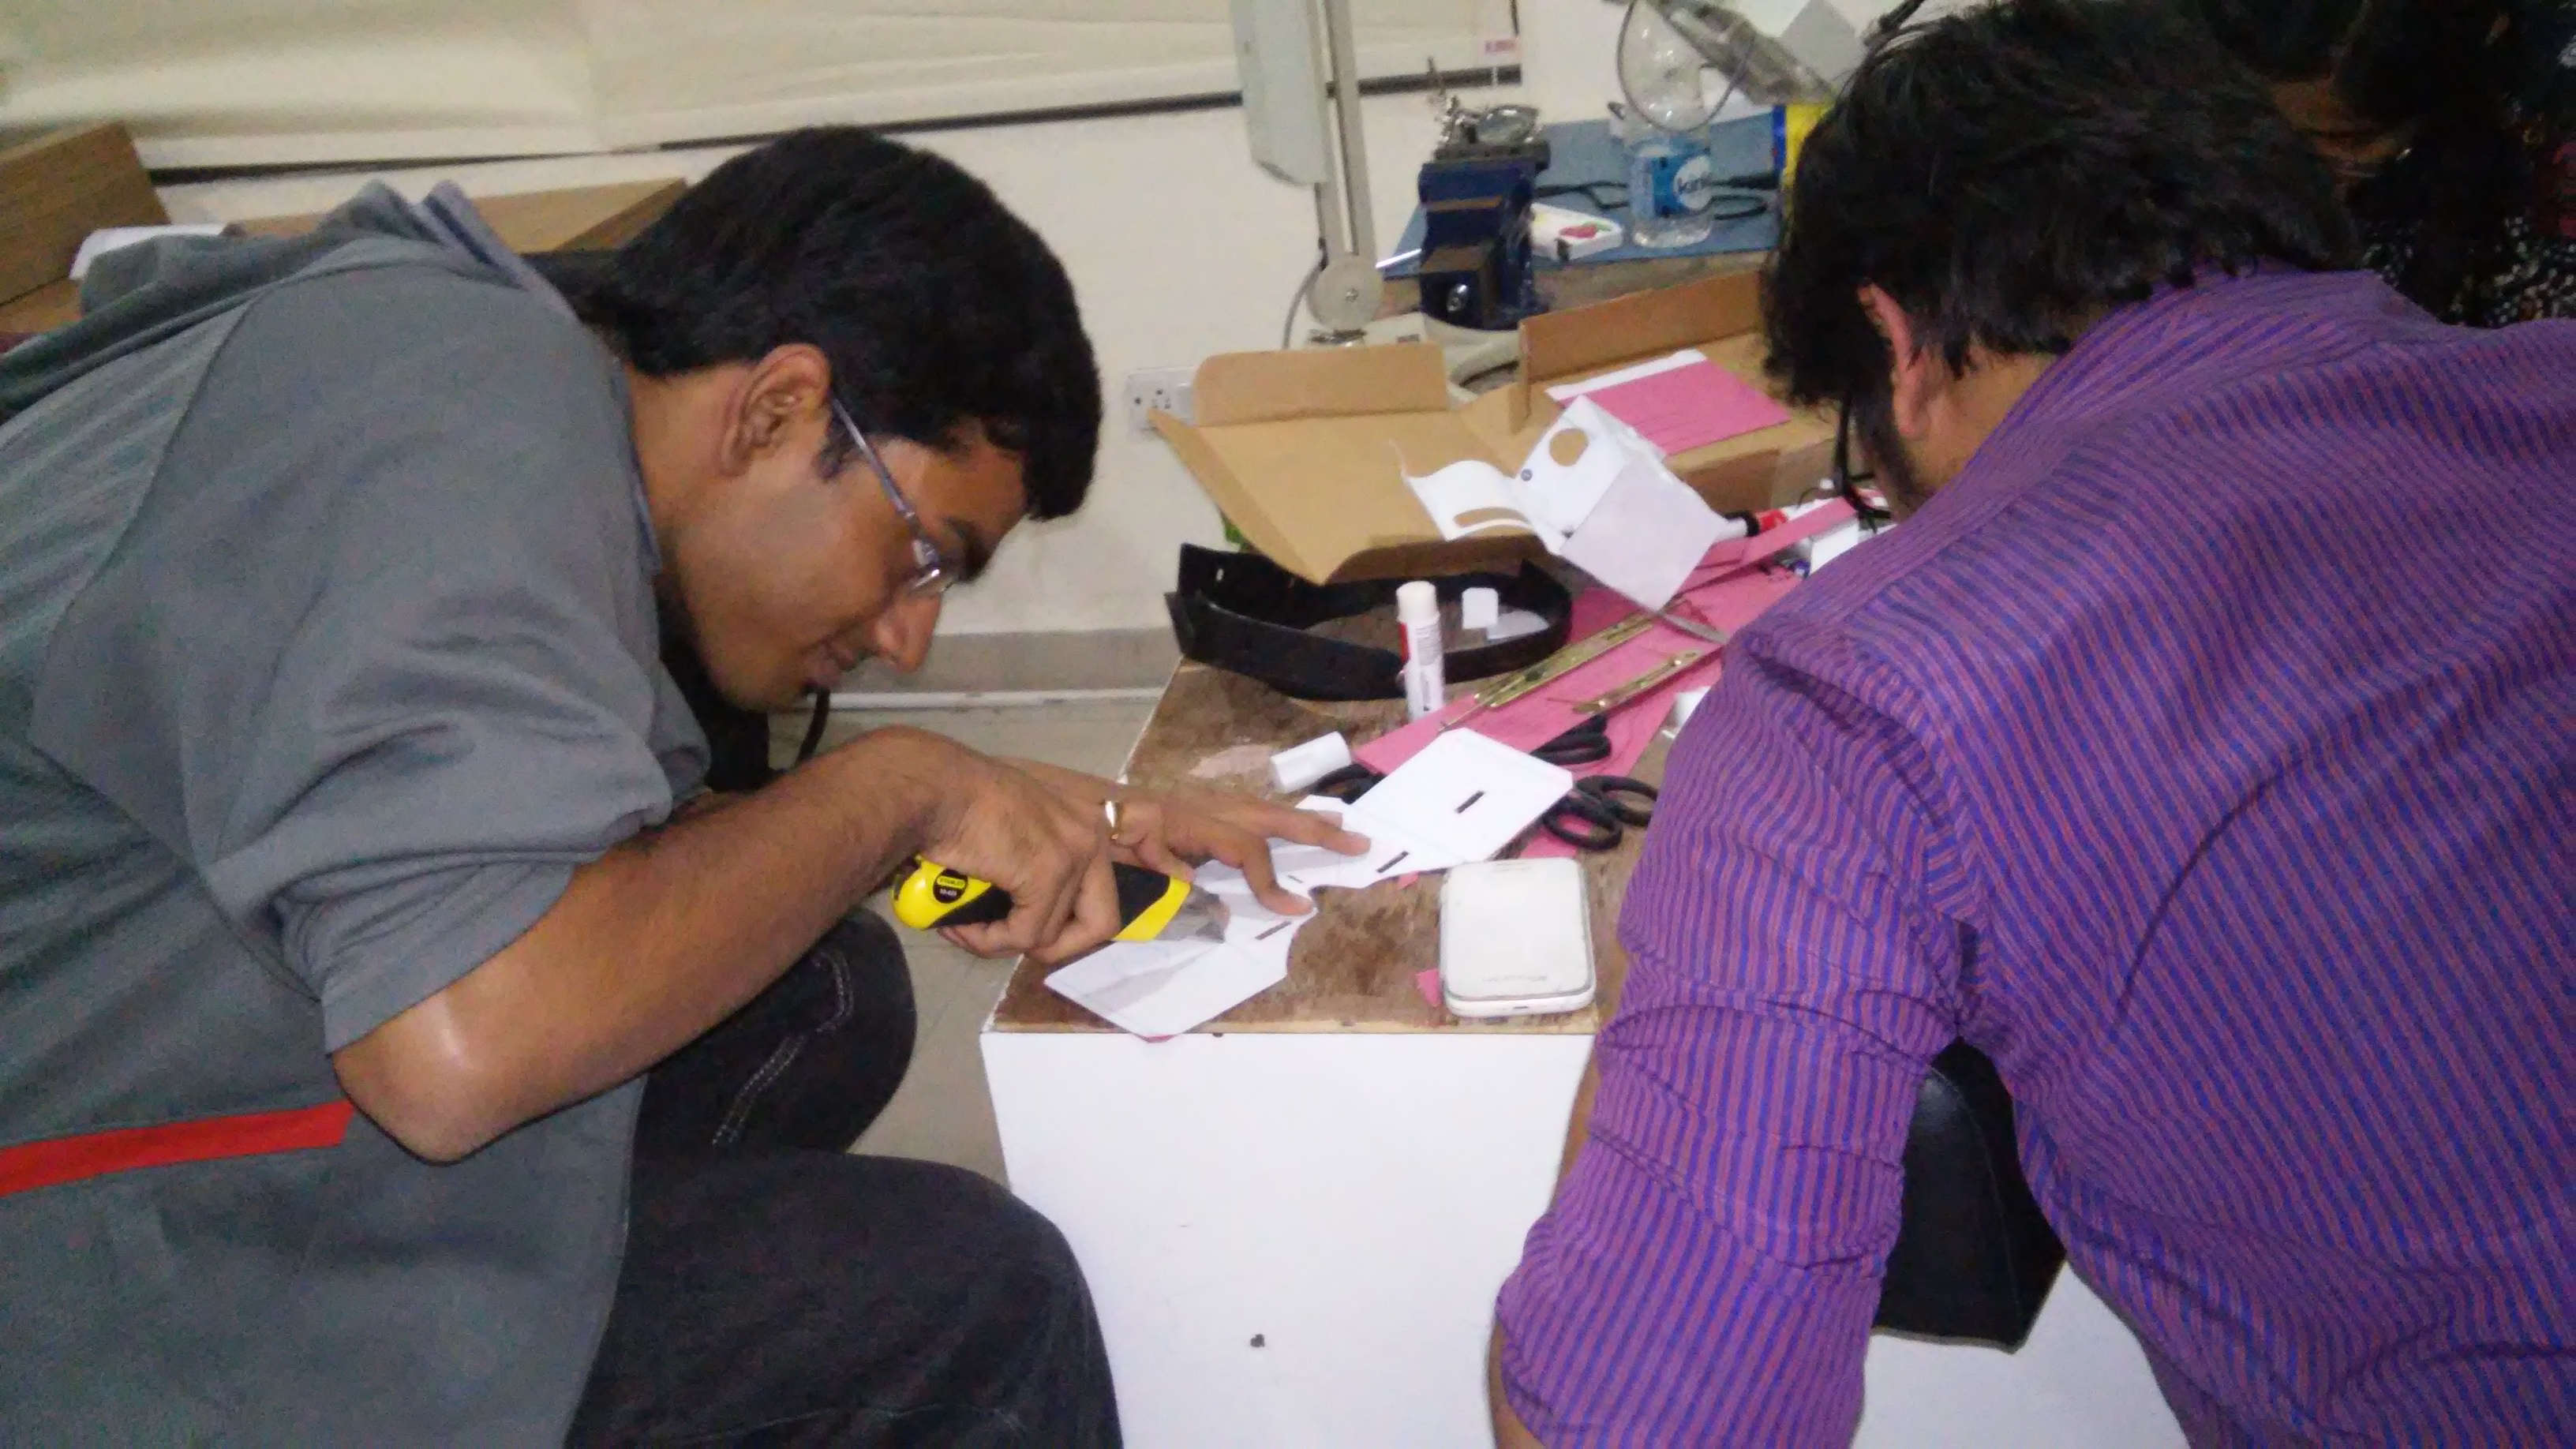
\includegraphics[width=8cm]{20141222_204533} 

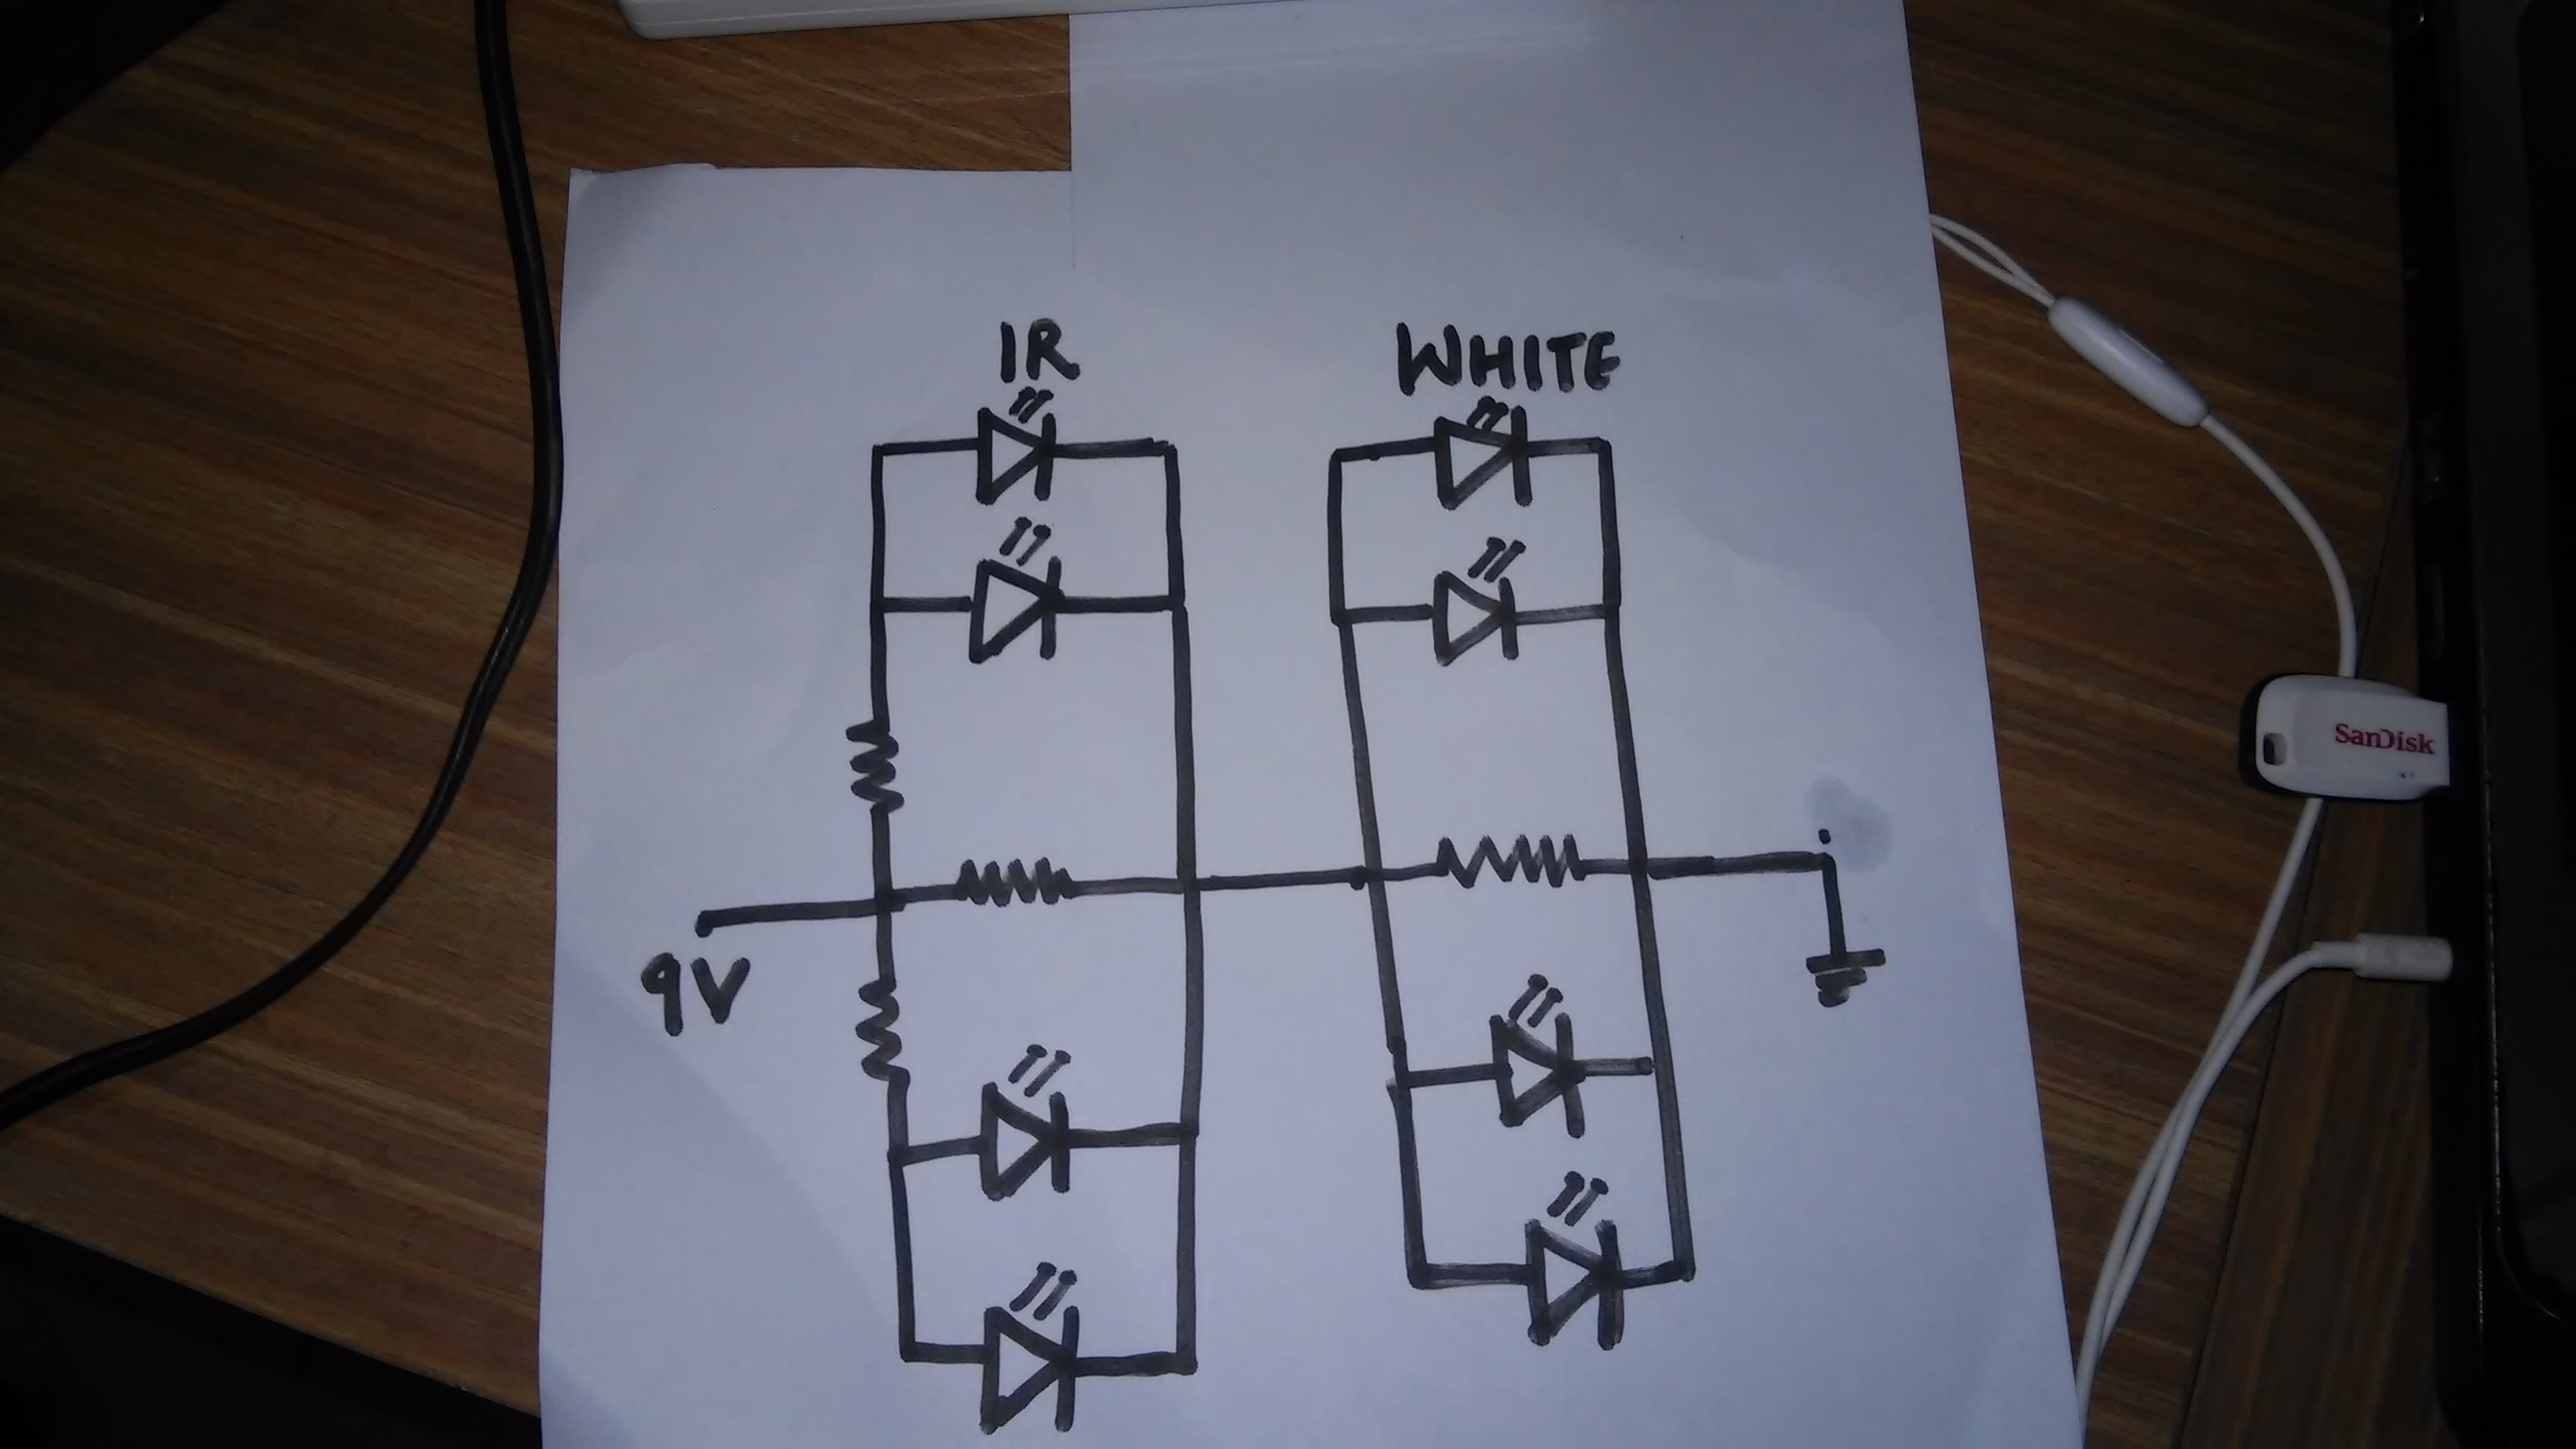
\includegraphics[width=8cm]{20141225_171833}
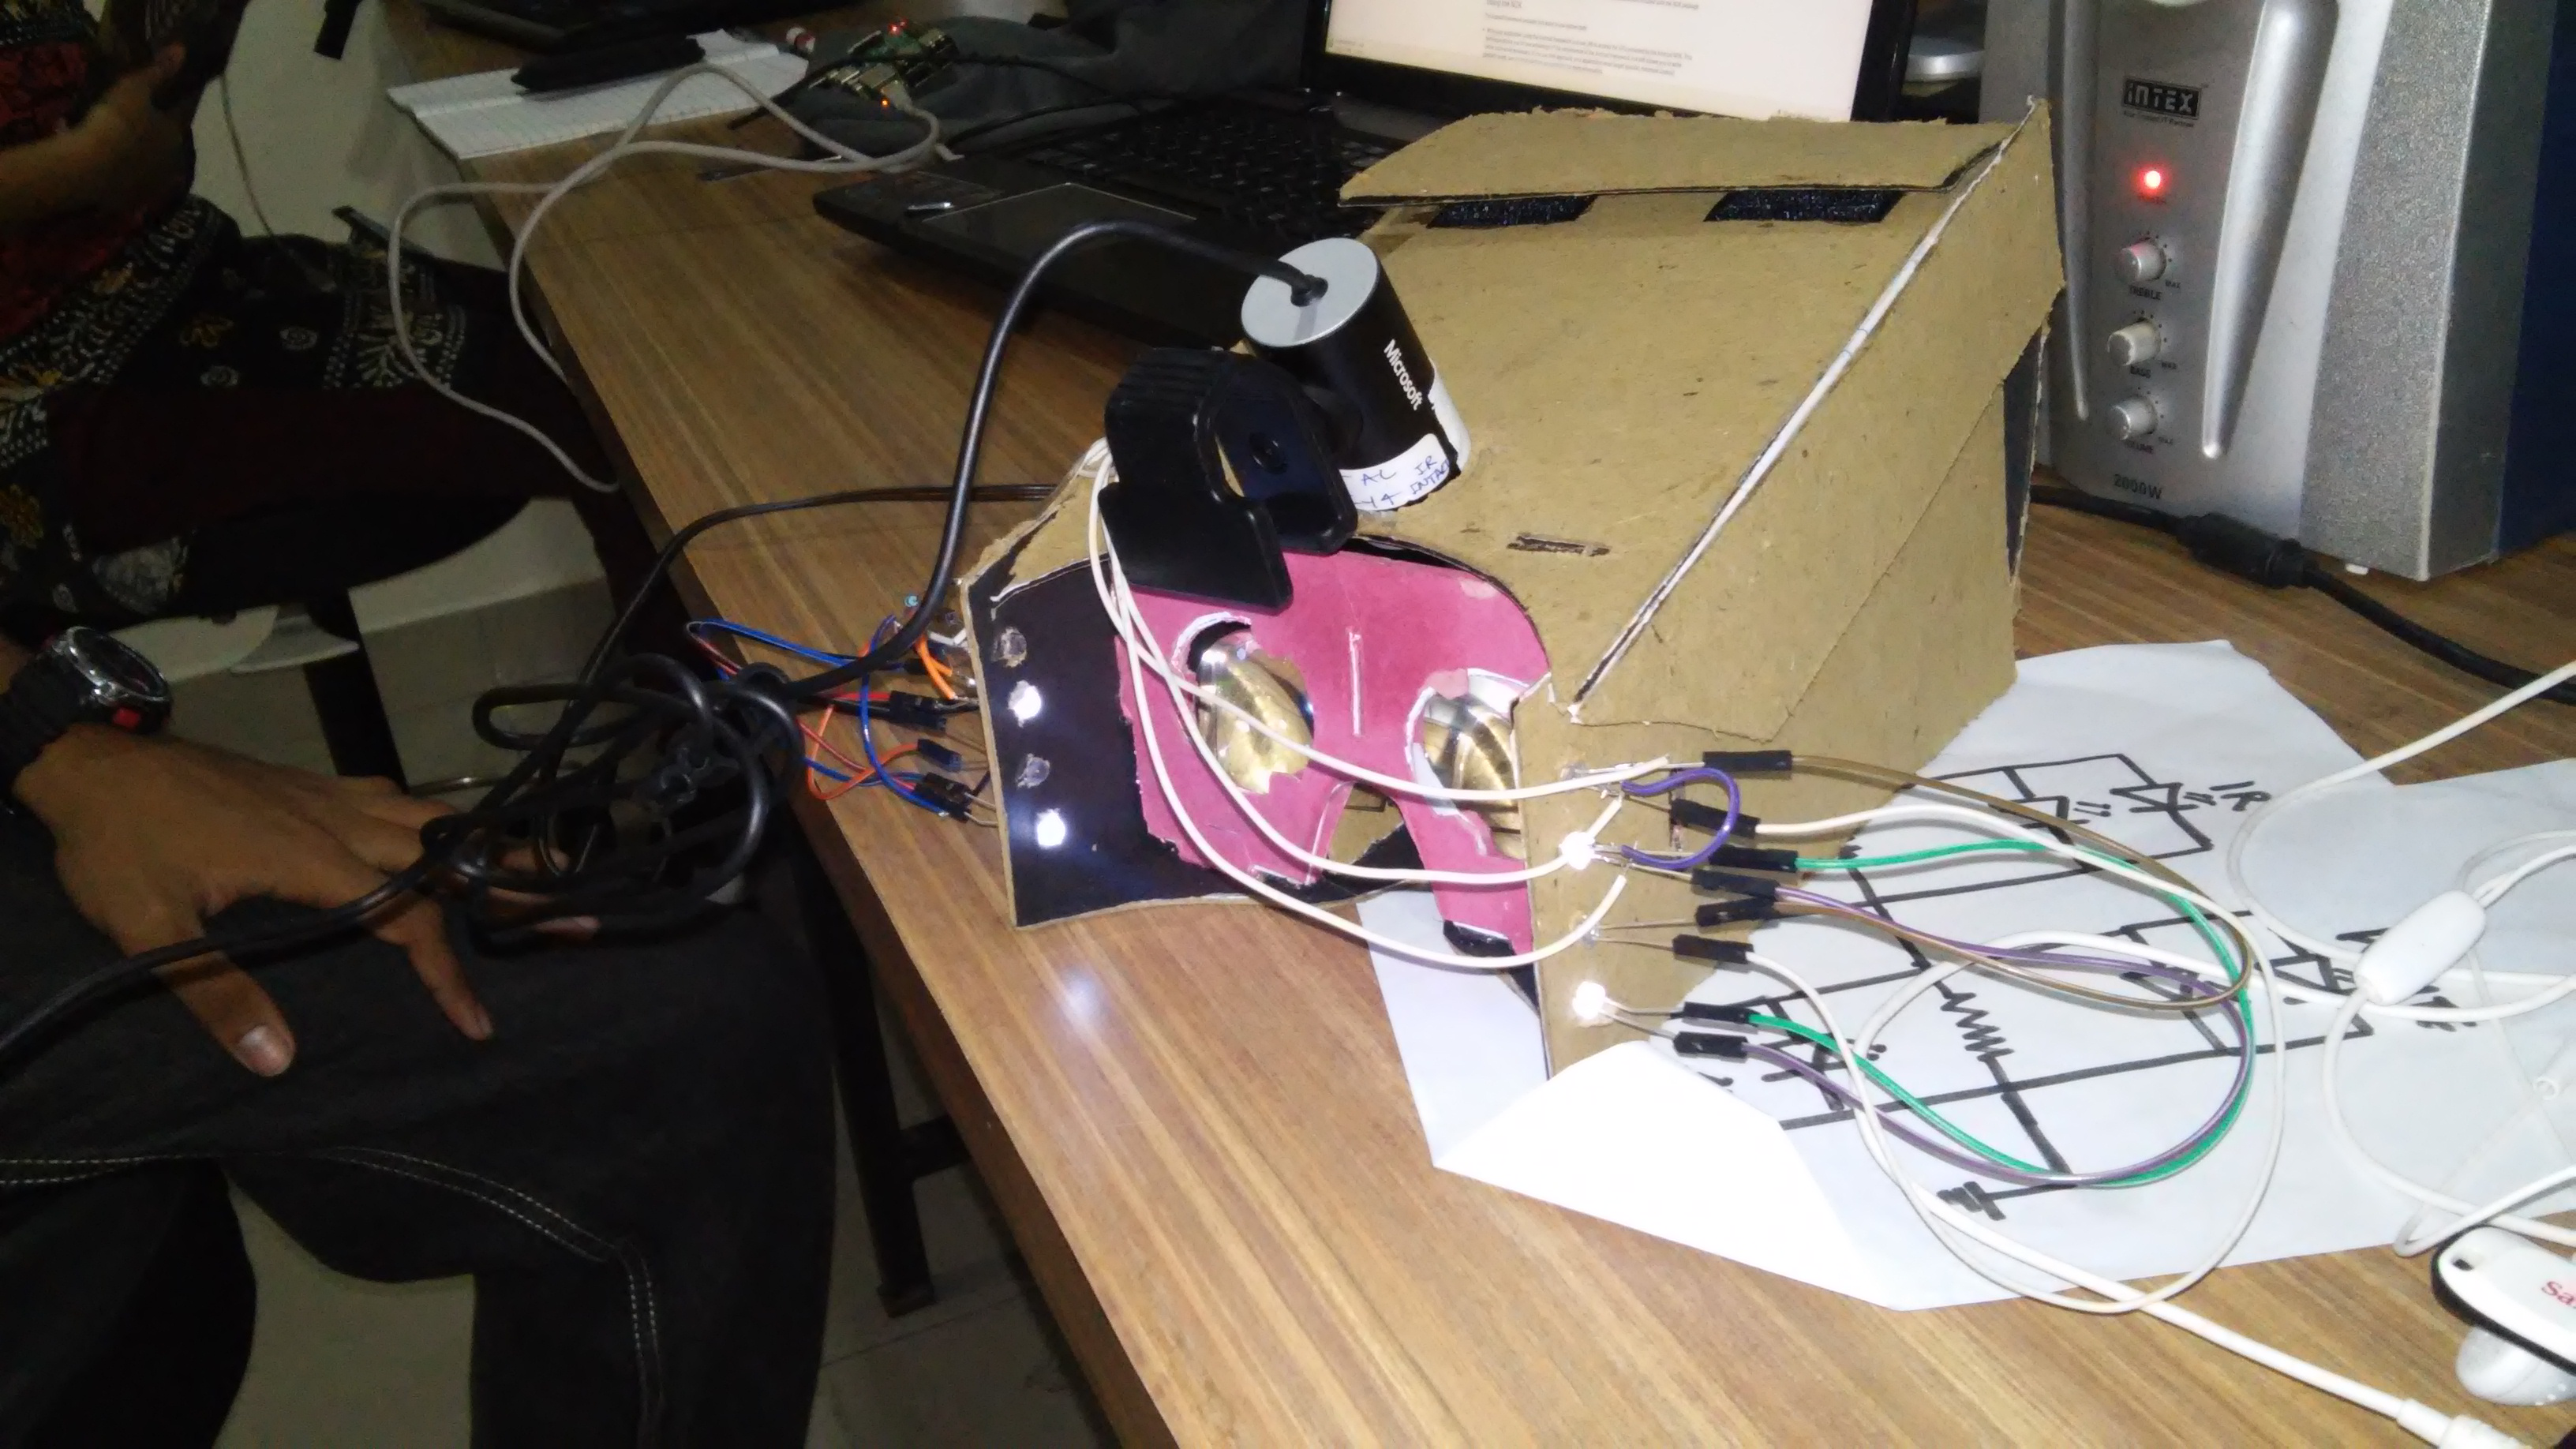
\includegraphics[width=8cm]{20141225_173411} 
\end{document}
